\documentclass[12pt]{beamer}
 
\usepackage[utf8]{inputenc}
\usepackage{tikz}

\usetheme{Madrid}
\usecolortheme{beaver}
 
%Information to be included in the title page:
\title[Lattice Cryptography]{Lattice Based Cryptography}
\author[Quinn Murphey]{Quinn Murphey}
\date[]{April 25, 2019}

%Presentation Topics
%
% Motivation
% Definition of Lattice
% Definition of Fundamental Domain and Lattice Cosets
% Probabilistic (7.5)
% Definition of SVP and CVP
% Babai’s Algorithm
% GGH Cryptosystem
% Relative Efficiency's with RSA and ECC
% If time, security 
% Further possibilities of lattices in a cryptosystem

\begin{document}
 
\frame{\titlepage}

\begin{frame}{Motivation}
    \frametitle{Why do we care about lattice based cryptography?}
    \begin{itemize}
        \item Significantly faster computations than both RSA and ECC
        \item Predicted to be "Quantum Proof" whereas RSA and ECC are already proven not to be.
        \item Provides a simple Fully Homomorphic Encryption Scheme
        \item Security from "worst-case" assumptions.
    \end{itemize}
\end{frame}

\begin{frame}{Lattices}
    \frametitle{Definitions}
    \begin{block}{Definition: Lattice}
        A Lattice is a discrete additive subgroup of $\mathbb{R}^n$.
    \end{block}
    \center
    \begin{tikzpicture}[scale = .9]
        \draw[black, thin, <->] (-2,0) -- (8,0);
        \draw[black, thin, <->] (0,-1) -- (0,4);
        \draw[black, thick, ->] (0,0) -- (3,0.5) node[midway,above,sloped] {$v_1$};
        \draw[black, thick, ->] (0,0) -- (.75,1.5) node[midway,below,sloped] {$v_2$};
        \filldraw[black] (0,0) circle (1.5pt);
        \filldraw[black] (3,0.5) circle (1.5pt);
        \filldraw[black] (6,1) circle (1.5pt);
        \filldraw[black] (3.75,2) circle (1.5pt);
        \filldraw[black] (6.75,2.5) circle (1.5pt);
        \filldraw[black] (1.5,3) circle (1.5pt);
        \filldraw[black] (2.25,4.5) circle (1.5pt);
        \filldraw[black] (4.5,3.5) circle (1.5pt);
        \filldraw[black] (7.5,4) circle (1.5pt);
        \filldraw[black] (0.75,1.5) circle (1.5pt);
        \filldraw[black] (2.25,-1) circle (1.5pt);
        \filldraw[black] (5.25,-.5) circle (1.5pt);
        \filldraw[black] (-2.25,1) circle (1.5pt);
        \filldraw[black] (-1.5,2.5) circle (1.5pt);
        \filldraw[black] (-.75,4) circle (1.5pt);
    \end{tikzpicture}
\end{frame}

\begin{frame}{Fundamental Domain}
    \frametitle{Definitions}
    \begin{block}{Definition: Fundamental Domain}
        The Fundamental Domain of a Lattice $\mathcal{L}$ with basis $\vec{v}_1,\vec{v}_2,\dots,\vec{v}_n$ is the set:
        $$\mathcal{F}(\mathcal{L}) = \{ t_1\vec{v}_1 + t_2\vec{v}_2 + \dots + t_n\vec{v}_n \space : \space 0\leq t_i < 1\}$$
    \end{block}
    \begin{columns}
        \begin{column}{.4\textwidth}
            Every vector $\vec{w}\in\mathbb{R}^n$ can uniquely be written $$\vec{w} = \vec{t} + \vec{v}$$ with $\vec{t}\in \mathcal{F}(\mathcal{L})$ and $\vec{v}\in \mathcal{L}$
        \end{column}
        \begin{column}{.6\textwidth}
            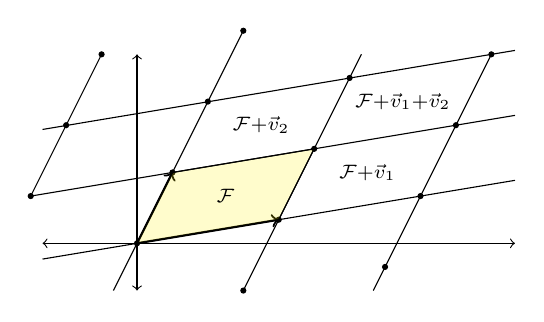
\begin{tikzpicture}[scale=0.6]
                \draw[black, thin, <->] (-2,0) -- (8,0);
                \draw[black, thin, <->] (0,-1) -- (0,4);
                \draw[black, thick, ->] (0,0) -- (3,0.5);
                \draw[black, thick, ->] (0,0) -- (.75,1.5);
                \filldraw[black] (0,0) circle (1.5pt);
                \filldraw[black] (3,0.5) circle (1.5pt);
                \filldraw[black] (0.75,1.5) circle (1.5pt);
                \filldraw[black] (6,1) circle (1.5pt);
                \filldraw[black] (3.75,2) circle (1.5pt);
                \filldraw[black] (6.75,2.5) circle (1.5pt);
                \filldraw[black] (1.5,3) circle (1.5pt);
                \filldraw[black] (2.25,4.5) circle (1.5pt);
                \filldraw[black] (4.5,3.5) circle (1.5pt);
                \filldraw[black] (7.5,4) circle (1.5pt);
                \filldraw[black] (2.25,-1) circle (1.5pt);
                \filldraw[black] (5.25,-.5) circle (1.5pt);
                \filldraw[black] (-2.25,1) circle (1.5pt);
                \filldraw[black] (-1.5,2.5) circle (1.5pt);
                \filldraw[black] (-.75,4) circle (1.5pt);
                \filldraw[thin, draw=black, fill=yellow, fill opacity=0.2] (0,0) -- (.75,1.5) -- (3.75,2) -- (3,.5) -- cycle;
                \draw[black, thin] (-0.5,-1) -- (2.25,4.5);
                \draw[black, thin] (2.25,-1) -- (4.75,4);
                \draw[black, thin] (5,-1) -- (7.5,4);
                \draw[black, thin] (-2.25,1) -- (-.75,4);
                \draw[black, thin] (-2.25,1) -- (8, 2.708);
                \draw[black, thin] (-2,2.41) -- (8,4.083);
                \draw[black, thin] (-2,-.33333) -- (8,1.33333);
                \draw[black] (1.875,1) circle (0pt) node[] {$\scriptstyle\mathcal{F}$};
                \draw[black] (2.625,2.5) circle (0pt) node[] {$\scriptstyle\mathcal{F} + \vec{v}_2$};
                \draw[black] (4.875,1.5) circle (0pt) node[] {$\scriptstyle\mathcal{F} + \vec{v}_1$};
                \draw[black] (5.625,3) circle (0pt) node[] {$\scriptstyle\mathcal{F} + \vec{v}_1 + \vec{v}_2$};
            \end{tikzpicture}
        \end{column}
    \end{columns}
\end{frame}

\begin{frame}{SVP and CVP}
    \frametitle{"Hard" Lattice Problems}
    $\lvert\lvert \vec{v}\rvert\rvert = \sqrt{x_1^2,x_2^2,\dots,x_n^2}$ where $x_i$ is the ith coordinate of $\vec{v}$ in $\mathbb{R}^n$.
    \begin{alertblock}{Shortest Vector Problem (SVP)}
        Find the shortest nonzero vector in a lattice $\mathcal{L}$. (Minimize $\lvert\lvert \vec{v}\rvert\rvert$)
    \end{alertblock}
    \begin{alertblock}{Closest Vector Problem (CVP)}
        Given a vector $\vec{w}\in\mathbb{R}^n$ not in $\mathcal{L}$, find the vector $\vec{v}\in\mathcal{L}$ which is closest to $\vec{w}$. (Minimize $\lvert\lvert \vec{w} - \vec{v}\rvert\rvert$)
    \end{alertblock}
    The \textit{expected shortest vector length} of a lattice $\mathcal{L}$ of dimension $n$ is
    $$\sigma(\mathcal{L}) = \sqrt{\frac{n}{2\pi e}}(\text{Vol}(\mathcal{F}))^{1/n} \approx 0.24197\sqrt{n}(\text{Vol}(\mathcal{F}))^{1/n}$$
\end{frame}

\begin{frame}{Babai's}
    \frametitle{Babai's Algorithm}
    Let $\mathcal{L}\subseteq\mathbb{R}^n$ be a $n$ dimensional lattice spanned by $\vec{v}_1,\vec{v}_2,\dots,\vec{v}_n$.
    \begin{block}{Babai's Algorithm}
        Given $\vec{w} = t_1\vec{v}_1 + t_2\vec{v}_2 + \dots + t_n\vec{v}_n \in R^n$, return $\vec{a}=\lfloor t_1\rceil\vec{v}_1 + \lfloor t_2\rceil\vec{v}_2 + \dots + \lfloor t_n\rceil\vec{v}_n$ as a likely closest vector.
    \end{block}
    
    Returns closest vertex of the Fundamental Domain which $\vec{w}$ is in.
    
    Does not work for "bad" basis, but is very likely to return the correct answer for a reasonably orthogonal basis.
    
\end{frame}

\begin{frame}{Good vs Bad Basis}
    \frametitle{Good vs Bad Basis}
    \begin{columns}[t]
        \begin{column}{.5\textwidth}
            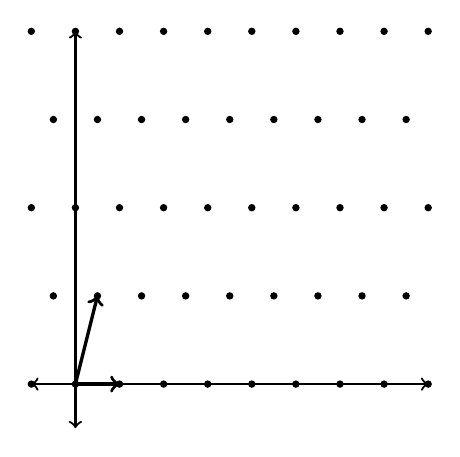
\begin{tikzpicture}[scale = .28]
                \draw[thick ,black, <->] (-2,0) -- (16,0);
                \draw[thick, black, <->] (0,-2) -- (0,16);
                \draw[very thick, black, ->] (0,0) -- (2,0);
                \draw[very thick, black, ->] (0,0) -- (1,4);
                \filldraw[] (-2, 16) circle (4pt);
                \filldraw[] (-2, 8) circle (4pt);
                \filldraw[] (-1, 12) circle (4pt);
                \filldraw[] (0, 16) circle (4pt);
                \filldraw[] (-2, 0) circle (4pt);
                \filldraw[] (-1, 4) circle (4pt);
                \filldraw[] (0, 8) circle (4pt);
                \filldraw[] (1, 12) circle (4pt);
                \filldraw[] (2, 16) circle (4pt);
                \filldraw[] (0, 0) circle (4pt);
                \filldraw[] (1, 4) circle (4pt);
                \filldraw[] (2, 8) circle (4pt);
                \filldraw[] (3, 12) circle (4pt);
                \filldraw[] (4, 16) circle (4pt);
                \filldraw[] (2, 0) circle (4pt);
                \filldraw[] (3, 4) circle (4pt);
                \filldraw[] (4, 8) circle (4pt);
                \filldraw[] (5, 12) circle (4pt);
                \filldraw[] (6, 16) circle (4pt);
                \filldraw[] (4, 0) circle (4pt);
                \filldraw[] (5, 4) circle (4pt);
                \filldraw[] (6, 8) circle (4pt);
                \filldraw[] (7, 12) circle (4pt);
                \filldraw[] (8, 16) circle (4pt);
                \filldraw[] (6, 0) circle (4pt);
                \filldraw[] (7, 4) circle (4pt);
                \filldraw[] (8, 8) circle (4pt);
                \filldraw[] (9, 12) circle (4pt);
                \filldraw[] (10, 16) circle (4pt);
                \filldraw[] (8, 0) circle (4pt);
                \filldraw[] (9, 4) circle (4pt);
                \filldraw[] (10, 8) circle (4pt);
                \filldraw[] (11, 12) circle (4pt);
                \filldraw[] (12, 16) circle (4pt);
                \filldraw[] (10, 0) circle (4pt);
                \filldraw[] (11, 4) circle (4pt);
                \filldraw[] (12, 8) circle (4pt);
                \filldraw[] (13, 12) circle (4pt);
                \filldraw[] (14, 16) circle (4pt);
                \filldraw[] (12, 0) circle (4pt);
                \filldraw[] (13, 4) circle (4pt);
                \filldraw[] (14, 8) circle (4pt);
                \filldraw[] (15, 12) circle (4pt);
                \filldraw[] (16, 16) circle (4pt);
                \filldraw[] (14, 0) circle (4pt);
                \filldraw[] (15, 4) circle (4pt);
                \filldraw[] (16, 8) circle (4pt);
                \filldraw[] (16, 0) circle (4pt);
            \end{tikzpicture}\\
            \center A "Good Basis"
        \end{column}
        \begin{column}{.5\textwidth}
            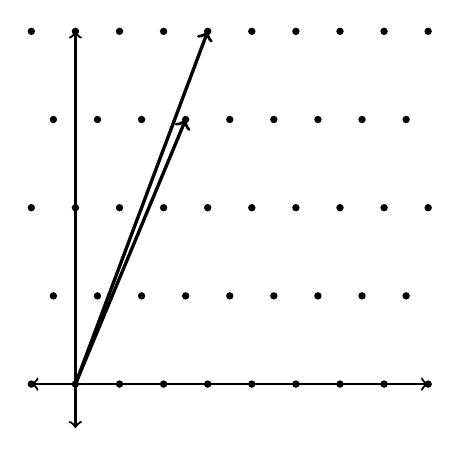
\begin{tikzpicture}[scale = .28]
                \draw[thick ,black, <->] (-2,0) -- (16,0);
                \draw[thick, black, <->] (0,-2) -- (0,16);
                \draw[very thick, black, ->] (0,0) -- (5,12);
                \draw[very thick, black, ->] (0,0) -- (6,16);
                \filldraw[] (-2, 16) circle (4pt);
                \filldraw[] (-2, 8) circle (4pt);
                \filldraw[] (-1, 12) circle (4pt);
                \filldraw[] (0, 16) circle (4pt);
                \filldraw[] (-2, 0) circle (4pt);
                \filldraw[] (-1, 4) circle (4pt);
                \filldraw[] (0, 8) circle (4pt);
                \filldraw[] (1, 12) circle (4pt);
                \filldraw[] (2, 16) circle (4pt);
                \filldraw[] (0, 0) circle (4pt);
                \filldraw[] (1, 4) circle (4pt);
                \filldraw[] (2, 8) circle (4pt);
                \filldraw[] (3, 12) circle (4pt);
                \filldraw[] (4, 16) circle (4pt);
                \filldraw[] (2, 0) circle (4pt);
                \filldraw[] (3, 4) circle (4pt);
                \filldraw[] (4, 8) circle (4pt);
                \filldraw[] (5, 12) circle (4pt);
                \filldraw[] (6, 16) circle (4pt);
                \filldraw[] (4, 0) circle (4pt);
                \filldraw[] (5, 4) circle (4pt);
                \filldraw[] (6, 8) circle (4pt);
                \filldraw[] (7, 12) circle (4pt);
                \filldraw[] (8, 16) circle (4pt);
                \filldraw[] (6, 0) circle (4pt);
                \filldraw[] (7, 4) circle (4pt);
                \filldraw[] (8, 8) circle (4pt);
                \filldraw[] (9, 12) circle (4pt);
                \filldraw[] (10, 16) circle (4pt);
                \filldraw[] (8, 0) circle (4pt);
                \filldraw[] (9, 4) circle (4pt);
                \filldraw[] (10, 8) circle (4pt);
                \filldraw[] (11, 12) circle (4pt);
                \filldraw[] (12, 16) circle (4pt);
                \filldraw[] (10, 0) circle (4pt);
                \filldraw[] (11, 4) circle (4pt);
                \filldraw[] (12, 8) circle (4pt);
                \filldraw[] (13, 12) circle (4pt);
                \filldraw[] (14, 16) circle (4pt);
                \filldraw[] (12, 0) circle (4pt);
                \filldraw[] (13, 4) circle (4pt);
                \filldraw[] (14, 8) circle (4pt);
                \filldraw[] (15, 12) circle (4pt);
                \filldraw[] (16, 16) circle (4pt);
                \filldraw[] (14, 0) circle (4pt);
                \filldraw[] (15, 4) circle (4pt);
                \filldraw[] (16, 8) circle (4pt);
                \filldraw[] (16, 0) circle (4pt);
    \end{tikzpicture}\\
            \center A "Bad Basis"
        \end{column}
    \end{columns}
\end{frame}

\begin{frame}{GGH}
    \frametitle{GGH Cryptosystem}
    Key Creation and Publishing:
    \begin{itemize}
        \item Private Key: "Good" basis for a lattice $\mathcal{L}$ ($\vec{v}_1,\vec{v}_2,\dots,\vec{v}_n$).
        \item Public Key: "Bad" basis for the same lattice ($\vec{w}_1,\vec{w}_2,\dots,\vec{w}_n$).
        \item Publish matrix $W$ with $\vec{w}_i$ as it's rows
    \end{itemize}
    Encryption:
    \begin{itemize}
        \item Choose small plaintext vector $\vec{m}\in\mathcal{L}$ and small ephemeral vector $\vec{r}\in\mathbb{R}^n$
        \item Ciphertext $\vec{e} = \vec{m}W + \vec{r}$
    \end{itemize}
    Decryption:
    \begin{itemize}
        \item Use Babai's algorithm with the good basis to find the closest $\vec{a}\in\mathcal{L}$ to $\vec{e}$, then compute $\vec{m} = \vec{a}W^{-1}$.
    \end{itemize}
\end{frame}

\begin{frame}{Comparisons}
    \frametitle{Comparisons with RSA and ECC}
    \begin{itemize}
        \item GGH has since been broken, but another unbroken system NTRU works similarly.
        \item NTRU has several orders of magnitude faster Encryption, Decryption, Key creation.
        \item ECC and RSA both have smaller keys and public parameters.
        
    \end{itemize}
    
\end{frame}

\begin{frame}{References}
    \frametitle{References}
    \begin{itemize}
        \item Hoffstein, Jeffery, Pipher, Jill, and Joseph H. Silverman, \textit{Introduction to Mathematical Cryptography}, SPRINGER-VERLAG NEW YORK, 2016, pp. 373–470.
        \item Nguyen, Hien Ba. “An Overview of the NTRU Cryptographic System.” San Diego State University, 2014. M.A. Thesis
        \item Peikert, Chris. \textit{A Decade of Lattice Cryptography}. Now Publishers, 2016.
        \item Hoffstein, Jeffery, et al. PUBLIC KEY CRYPTO-SYSTEM METHOD AND APPARATUS. 27 June 2000. US-6,081,597
    \end{itemize}
    
    
\end{frame}

\end{document}
